%
%                                %
%                             %
%                          %
%      %                %     %
%         %          %           %
%            %    %                 %
%               %                      %
%                  %                 %    %
%                     %           %          %
%                        %     %                %
%                           %
%                        %
%                     %
%                  %
%
%                     In Math We Trust
%            Quaternion Church: All rights reserved

\documentclass[aspectratio=1610]{beamer}
\hypersetup{
    unicode = true,
    linkcolor = blue,
    anchorcolor = blue,
    citecolor = green,
    filecolor = black,
    urlcolor = blue
}
\usefonttheme{professionalfonts}
\usepackage{amsmath}
\usepackage{amssymb}
\usepackage{caption}
\usepackage{fvextra}
\usepackage{csquotes}
\usepackage{listings}
\usepackage{lmodern}
\usepackage[cache=false]{minted}
\usepackage{textcomp}
\usepackage{xcolor}
\usepackage{tikz}
\usepackage{bm}
\usepackage{fix-cm}
\usetikzlibrary{arrows.meta}
\usetikzlibrary{decorations.pathreplacing}
\usetikzlibrary{positioning,calc}
\usepackage{graphicx}
\usepackage{hyperref}
\usepackage{listings}
\usepackage{fontawesome}
\usepackage[english]{babel}
\usepackage[backend=biber, style=numeric]{biblatex}
\setbeamertemplate{frametitle continuation}{}

\input{smile_styles}
\renewcommand{\thefootnote}{\fnsymbol{footnote}}
\addbibresource{references.bib}
\title{Improving the Minkowski Constant Using the Exponent of Decay}\author{Rongqing Wang, Zhongyi Li, Tianer Tang}
\date\today
\begin{document}
\begin{frame}[plain]
    \titlepage
    \vfill
    \centering
    \small Guided by Professor Nikolay Moshchevitin
\end{frame}
\begin{frame}{Contents}\tableofcontents\end{frame}

\section{Introduction}
\subsection{1.1 Introduction to Multidimensional Diophantine Approximation}
\begin{frame}
    \frametitle{1.1 Introduction to Multidimensional Diophantine Approximation}
    To approximate an irrational vector $\boldsymbol{\alpha} \in \mathbb{R}^d \setminus \mathbb{Q}^d$ with integer vectors under a norm $\|\cdot\|$:
    %Say: There's more than one way of approximating our vector alpha.
    \begin{itemize}        
        \item \textbf{Linear Form Approximation (LF)}: $(\mathbf{q},p) \in \mathbb{Z}^d \times \mathbb{Z} \setminus      \{\textbf{0}\}$ which minimize $| \mathbf{q} \cdot \boldsymbol{\alpha} - p | = |q_1\alpha_1 + \dots + q_d\alpha_d - p|$
        \item \textbf{Simultaneous Approximation (SA)}: $(q,\mathbf{p}) \in \mathbb{Z}^+ \times \mathbb{Z}^d$ 
            which minimize $ \|q\boldsymbol{\alpha} - \mathbf{p}\|$
    \end{itemize}

    In this presentation we will work with two-dimensional LF approximations under the Euclidean norm.\vspace{0.6cm}\\
    Require $1, \alpha_1, \alpha_2$ linearly independent over $\mathbb{Q}$.

        \begin{definition}[Minkowski Constant for two-dimensional LF]
        A positive constant $c$ such that for any $\boldsymbol{\alpha}$ there exist infinitely many approximations $(\mathbf{q},p) \in \mathbb{Z}^3$ which satisfy $| \mathbf{q} \cdot \boldsymbol{\alpha} - p | < \dfrac{1}{c\|\textbf{q}\|^2}$.
    \end{definition}
\end{frame}

\begin{frame}
    \frametitle{Geometrical Interpretation}
    \begin{theorem}[Minkowski, \cite{minkowski1893convex}]
        Let $A \subset \mathbb{R}^3$ be a set which is convex and symmetric about the origin. If 
        $\mathrm{vol}(A)>2^3,$ then $A$ contains a nonzero point in $\mathbb{Z}^3$.
    \end{theorem}
    \vspace{0.5cm}
    For positive constants $c_l$, $c_s$, define the following sets:
    \[
        S_l := \left\{(x_1,x_2, y)\in \mathbb{R}^3:\ |\alpha_1x_1 + \alpha_2x_2-y| < \frac{1}{c_l\|(x_1,x_2)\|^2}\right\}
    \]
    %  这玩意是对平面的逼近
    % We notice that the expression on the LHS has a geometrical interpretation of the vertical distance to an irrational plane
    \pause
    \[
        S_s := \left\{(y_1, y_2, x)\in \mathbb{R}^3: \ \|(\alpha_1x - y_1, \alpha_2x-y_2)\| < \frac{1}{c_s\sqrt{|x|}}\right\}
    \]
    % 这玩意是对直线的逼近
    % We notice again that the expression on the LHS has a geometrical interpretation of the horizontal distance to an irrational line
    \[
        S := \left\{(x, y, z):\ \|(x,y)\|^2|z|<\frac{1}{k}\right\}
    \]
    % 这是介俩玩意儿的共同形式
    % And if we rearrange the terms, and take the square of the SA part, remember that square,
    %we can find that they actually share the same form as S. Now you are actually seeing the duality between LF and SA! Algebraicly, if we let :) = :| = :(, we will get the same sets, and next we will formalize this and provide a geometrical view of this duality.
    \\
    %Say: We notice that they share a same form if we multiply by denominators and taking square of S_s. This is the inspiration of duality between SA and LF. Specifically, as we'll see later, the duality between the sets of good approximations. (Not best approximation vectors! Even not good approximation vectors!!)
\end{frame}

\subsection{1.2 Duality between two-dimensional LF and SA}
\begin{frame}
    \centering
    \begin{tikzpicture}[every node/.style={inner sep=0pt}]
        \node (LF) {
            \includegraphics[width=0.26\textwidth]{LF.png}
        };
        \node[yshift=-48pt] at (LF) {$S_l$};
        \node[right=4cm of LF] (STD){
            \includegraphics[width=0.26\textwidth]{STANDARD.png}
        };
        \node[yshift=-48pt] at (STD) {$S$};
        \node[below=0.5cm of STD] (SA){ 
            \includegraphics[width=0.26\textwidth]{SA.png}
        };
        \node[yshift=-48pt] at (SA) {$S_s$};

        \draw[->, thick] (LF) -- node[above, yshift=3pt] {
            $\chi^\top$
        } (STD);
        \draw[->, thick] (SA) -- node[right, xshift=3pt] {
            $\chi$
        } (STD);
        \node[right] at (-3, -3.5) {
            Choose $c_s^2 = k = c_l$:
        };
        \node[right] at (-3,-4.7) {
            $\displaystyle \chi=\begin{bmatrix}1&&-\alpha_1\\&1&-\alpha_2\\ &&1\end{bmatrix}$,
        };
        \node[right] at (0.5,-4.7) {
            $\displaystyle \chi^\top=\begin{bmatrix}1&&\\&1&\\-\alpha_1&-\alpha_2&1\end{bmatrix}$
        };
    \end{tikzpicture}
    % Now we have plotted the Sl , S and Ss. As I've promised, Sl is like approximating a plane -- the "base" of the set, while Ss is like approximating a line -- the "axis" of the set. Remember the change of variable on the privious slide? Tthese two big matrices is just a notation for that changement of variables. Remember that square we took on SA? Here it becomes the first equality describing the relationships between the LF const and the SA const. Keep that in mind and we will meet him in a moment.
\end{frame}

\section{Derivation of the Improved Minkowski Constant }
\subsection {2.1 Best Approximations}
\begin{frame}{2.1 Best Approximations}
    For vector $\boldsymbol{\alpha}=(\alpha_1, \alpha_2)$ with $1, \alpha_1, \alpha_2$ linearly independent over $\mathbb{Q}$,
    we have a sequence of approximation vectors called `Best Approximations'
    \[
        (\textbf{q}_\nu, p_\nu) = (q_{1,\nu}, q_{2,\nu}, p_\nu) \in \mathbb{Z}^{3}\setminus \{\textbf{0}\}
    \]
    with the property that for the approximation error $\delta_\nu =|\textbf{q}_\nu \cdot \boldsymbol{\alpha} - p_\nu|$ holds
    \[
        \delta_\nu < |\textbf{q}\cdot\boldsymbol{\alpha} - p|
    \]
    for any vector $\textbf{q} \in \mathbb{Z}^2 \setminus \{\textbf{0}\}$ with $\|\textbf{q}\|<\|\textbf{q}_\nu\|$.
    %Say: We arrange such a sequence of best approximations in order of strictly increasing q_nu.
    %     Consecutive best approximation vectors exhibit a particularly useful trait:
    \begin{lemma}[Empty Pie]
        Define $\Pi := \left\{(x_1, x_2, y) \in \mathbb{R}^3: \ \|(x_1, x_2)\| < \|\textbf{q}_{\nu+1}\|, |x_1\alpha_1 + x_2\alpha_2 - y| < \delta_\nu \right\}$.
        Then $\Pi_\nu$ contains no nonzero lattice points.
    \end{lemma}
    %Say: This lemma actually plays a key role in two totally different parts of our proof.
\end{frame}

\subsection{2.2 Main Proof}
\begin{frame}{2.2 Main Proof}
\centering
\begin{tikzpicture}[xscale=1.618,yscale=0.9,>=Stealth,font=\footnotesize]
    \coordinate (A) at (-2,0);
    \coordinate (B) at (-2,-4);
    \coordinate (C) at (2,0);
    \coordinate (D) at (2,4);
    \coordinate (znu)  at (1,3);
    \coordinate (znu1) at (2,1);
    
    \only<1>{%
        \begin{scope}
            \fill[gray!10](1,-1) -- (1,0) -- (2,1) -- (2,3) -- (1,2) -- (1,3)-- (-1,1) -- (-1,0) -- (-2,-1) -- (-2,-3) -- (-1,-2) -- (-1,-3) -- cycle;
            \fill[gray!20] (1,-1) -- (1,0) -- (-1,-2) -- (-1,-3) -- cycle;
            \fill[gray!20] (1,2) -- (1,3) -- (-1,1) -- (-1,0) -- cycle;
            \draw[dotted] (-1,-2) -- (-1,1);
            \draw[dotted] (1,-1) -- (1,3);
            \draw (A) -- (B) -- (C) -- (D) -- cycle;
            \draw[dotted] (2,1) -- (2,3) -- (-2,-1) -- (-2,-3) -- cycle;
            \node[right] at (-4, 3) {
                $\Pi_\nu := \{(\textbf{x}, y): \|(x_1, x_2)\| < \|\textbf{q}_{\nu+1}\|,$
            };
            \node[right] at (-2.68, 2.4) {
                $|x_1\alpha_1 + x_2\alpha_2 - y| < \delta_\nu \}$
            };
            \node[right] at (1.4,-0.8) {
              \textit{Empty Pie} says that two
            };
            \node[right] at (1.4,-1.4) {
              consecutive B.A. vectors
            };
            \node[right] at (1.4,-2) {
              define a region free of
            };
            \node[right] at (1.4,-2.6) {
              nonzero lattice points.
            };
        \end{scope}%
    }

    \only<1-2>{%
        \begin{scope}
            \draw[->] (0,0) -- (znu)  node[yshift=10pt,xshift=-2pt, font=\footnotesize] {
                $(\mathbf{q}_\nu, p_\nu)$
            };
            \draw[->] (0,0) -- (znu1) node[xshift=25pt, font=\footnotesize] {
                $(\mathbf{q}_{\nu+1}, p_{\nu+1})$
            };
        \end{scope}%
    }

    \only<2>{%
        \begin{scope}
            \node[right] at (-4,3) {
                $S := \left\{(\textbf{x}, y):\ |\boldsymbol{\alpha}\cdot \textbf{x}-y| < \frac{1}{c\|\textbf{x}\|^2}\right\}$
            };
        \end{scope}%
        \node[right] at (1.4,-0.8) {
            If there are infinitely many
        };
        \node[right] at (1.4,-1.4) {
            vectors $(\textbf{q}_\nu , p_\nu)$ within $S$,
        };
        \node[right] at (1.4,-2) {
            we're done.
        };
        \node[right] at (1.4,-2.8) {
            Else $\forall \nu > T$, $(\textbf{q}_\nu , p_\nu)\not \in S$
        };
    }
  
    \only<2->{%
        \begin{scope}
            \draw[domain=0.5:3,blue,smooth,variable=\x]
                plot ({\x},{\x + 1.618/\x});
            \draw[domain=0.5:3,blue,smooth,variable=\x]
                plot ({\x},{\x - 1.618/\x});
                
            \draw[dotted] (A) -- (B) -- (C) -- (D) -- cycle;
            \draw[dotted] (2,1) -- (-2,-3);
            \draw[dotted] (2,3) -- (-2,-1);
        \end{scope}
    }

    \only<3->{%
      \begin{scope}
        \draw[domain=0:2.   427] plot (\x,-0.236*\x+3);
        \draw[domain=0:2.427] plot (\x,2.236*\x-3);
        \draw [decorate,decoration={brace,amplitude=6pt}]
            (0.809,0.809) -- (0.809,2.809)
            node [black,midway,xshift=-13pt,font=\tiny] {$\delta_\nu$};
        \draw [decorate,decoration={brace,amplitude=6pt}]
            (1.618,1.618) -- (1.618,2.618)
            node [black,midway,xshift=-16pt,yshift=-2pt,font=\tiny] {$\delta_{\nu+1}$};
      \end{scope}%
    }

    \only<4>{%
        \begin{scope}
            \draw[domain=-3:-0.55,red,variable=\x] plot ({\x},{\x + 1.820/\x});
            \draw[domain=-3:-0.55,red,variable=\x] plot ({\x},{\x - 1.820/\x});
            \draw[domain=0.55:3,red,variable=\x] plot ({\x},{\x + 1.820/\x});
            \draw[domain=0.55:3,red,variable=\x] plot ({\x},{\x - 1.820/\x});
        \end{scope}
    }

    \only<4->{%
        \begin{scope}
            \draw[domain=-3:-0.5,blue,smooth,variable=\x] plot ({\x},{\x + 1.618/\x});
            \draw[domain=-3:-0.5,blue,smooth,variable=\x] plot ({\x},{\x - 1.618/\x});
            \draw[domain=-2.427:0] plot (\x,-0.236*\x-3);
            \draw[domain=-2.427:0] plot (\x,2.236*\x+3);
        \end{scope}%
    }

    \only<5->{%
        \begin{scope}
            \draw [decorate,decoration={brace,amplitude=7pt}]
                (0,0) -- (2.427,0)
                node [black,midway,yshift=12pt] {$R$};
            \draw [decorate,decoration={brace,amplitude=7pt}]
                (0,0) -- (0,3)
                    node [black,midway, xshift=-12pt] {$H$};
            \draw[dotted] (2.427,2.427) -- (2.427,0);
            \node[right, font=\Tiny] at (1.7,-1) {
               $\displaystyle R=\frac{\delta_\nu \delta_{\nu+1}^{-\frac{1}{2}}-\delta_{\nu+1} \delta_{\nu}^{-\frac{1}{2}}}{\sqrt{c}(\delta_\nu-\delta_{\nu+1})}$
            };
            \node[right, font=\Tiny] at (1.7,-2) {
               $\displaystyle H=\frac{\delta_\nu \delta_{\nu+1}^{-\frac{1}{2}}-\delta_{\nu+1} \delta_{\nu}^{-\frac{1}{2}}}{\delta_{\nu+1}^{-\frac{1}{2}}-{\delta_\nu^{-\frac{1}{2}}}}$
            };
            \node[right] at (1.7,-3.2) {
               $\mathrm{vol}(A)=\frac{2\pi}{3} R^2 H >8$
            };
        \end{scope}%
    }
    \draw (3,3) -- (-3,-3); %y = alpha x
    \draw[->] (0,-4) -- (0,4);
    \node[left] at (0,4) {$y$};
    \draw[->] (-3,0) -- (3,0);
    \node[below] at (3,0) {$\bm{\mathbf{x}}$};
    \node[below] at (3,0) {$\textbf{x}$};
    % Clip to frame area
    \clip (-4,-4) rectangle (4,4);
\end{tikzpicture}
\end{frame}

\subsection{2.3 Results}
\begin{frame}{2.3 Results}
  \begin{lemma}[Kissing Number Lemma\cite{Ermakov2010}]
    \[\forall \nu\in \mathbb{Z}^+:\ \delta_\nu > \delta_{\nu+5} + \delta_{\nu+6}\]
  \end{lemma}
  \medskip
  As a corollary, $\exists$ infinitely many $\nu$ with $\delta_\nu > t \cdot \delta_{\nu+1}$, where $t^6 - t - 1 = 0:\ t \approx 1.134^+$

  \medskip

  Computations show that $\displaystyle c = \frac{\pi}{12} \cdot \frac{\big(t - t^{-1/2}\big)^3}{(t-1)^2\big(1 - t^{-1/2}\big)}$
  guarantees $\mathrm{vol}(A) > 8$ for all such $\nu$.

  By \textit{Minkowski}, we have found a lattice point within $A$ and $S$.
  Vary $\nu$ to find infinitely many such points.

  \[c \approx 1.772^+ > 1.767^+ = \frac{9\pi}{16}\footnote[2]{\textit{We call an improvement like this ‘too bad to be false’}}\]

\end{frame}

\subsection{2.4 Generalization}
\begin{frame}{2.4 Generalization}
    %Say: The generalization from two-dimensional linear form approximations in the Euclidean norm to an arbitrary dimension, and norm, and simultaneous approximations, can be accomplished by the following few observations.
    \begin{itemize}
        \item Euclidean norm $\rightarrow$ Any norm
        \item $\boldsymbol{\alpha} \in \mathbb{R}^2 \rightarrow     \boldsymbol{\alpha} \in \mathbb{R}^d$
        \item Linear Form Approximation $\rightarrow$ Simultaneous Approximation
    \end{itemize}
    %Say: Norms stay convex in any dimensions
    %     Homotheties still occur between parallel balls in any dimensions.
    %     We present the following formula derived for the general case:
    $v=\mathrm{vol}(B_N^d(1))$ and $t>1$ is the exponent of decay.
    %Say: where v is the volume of the d-dimensional unit ball and t is the exponent of decay of best approximation remainders.
    \[
        c=\dfrac{v\left(t-t^{-\frac{1}{d}}\right)^{d+1}}{2^d(d+1)(t-1)^d\left(1-t^{-\frac{1}{d}}\right)} > \dfrac{v}{2^d}\left(\dfrac{d+1}{d}\right)^d
    \]
    %Say: Surprisingly to us, the formula for simultaneous approximations looks almost the exact same except an exponent of dimension.
    \pause
    \[
        c_s=\sqrt[d]{\dfrac{v\left(t_s-t_s^{-\frac{1}{d}}\right)^{d+1}}{2^d(d+1)(t_s-1)^d\left(1-t_s^{-\frac{1}{d}}\right)}} > \sqrt[d]{\dfrac{v}{2^d}}\dfrac{d+1}{d}
    \]
\end{frame}

\section{Future Plans}
\begin{frame}{3 Future Plans}
    \begin{itemize}
        \item Generalize this method to general approximation case $\|\Theta\mathbf{q}-\mathbf{p}\|$ where $\Theta\in\mathbb{R}^{n\times m}$, and $\mathbf{q}\in\mathbb{Z}^m,\mathbf{p}\in\mathbb{Z}^n$.
        \item Combine this method with \textit{Minkowski} for non-convex  bodies to get better results\cite{Moshchevitin2002}.
        \item Improve the exponent of decay of LF approximation because that benefits our result.
    \end{itemize}
\end{frame}

\addtobeamertemplate{frametitle}{}{%
    \vspace*{-1.5em}
}

\section{Reference}
\begin{frame}[allowframebreaks]
    \frametitle{References}
    \printbibliography
    \begin{center} 
        \Huge Thank You!
    \end{center} 
\end{frame}

\end{document}